%% Modelo adaptado de abtex2-modelo-trabalho-academico.tex, v-1.8 laurocesar
%% Copyright 2012-2013 by abnTeX2 group at http://abntex2.googlecode.com/ 
%%
%% This work may be distributed and/or modified under the
%% conditions of the LaTeX Project Public License, either version 1.3
%% of this license or (at your option) any later version.
%% The latest version of this license is in
%%   http://www.latex-project.org/lppl.txt
%% and version 1.3 or later is part of all distributions of LaTeX
%% version 2005/12/01 or later.
%%
%% This work has the LPPL maintenance status `maintained'.
%% 
%% The Current Maintainer of this work is the abnTeX2 team, led
%% by Lauro César Araujo. Further information are available on 
%% http://abntex2.googlecode.com/

%%******************************************************
%%******************************************************
%% This work consists of the files:
%% abntex2-modelo-trabalho-academico-TCC-EngaEletrica.tex,
%% abntex2-modelo-include-comandos 
%% abntex2-modelo-references.bib
%%******************************************************
%%******************************************************

% ------------------------------------------------------------------------
% ------------------------------------------------------------------------
% abnTeX2: Modelo de Trabalho Academico (tese de doutorado, dissertacao de
% mestrado e trabalhos monograficos em geral) em conformidade com 
% ABNT NBR 14724:2011: Informacao e documentacao - Trabalhos academicos -
% Apresentacao
% ------------------------------------------------------------------------
% ------------------------------------------------------------------------

\documentclass[
	% -- opções da classe memoir --
	12pt,				% tamanho da fonte
	openright,			% capítulos começam em pág ímpar (insere página vazia caso preciso)
	twoside,			% para impressão em verso e anverso. Oposto a oneside
	a4paper,			% tamanho do papel. 
	% -- opções da classe abntex2 --
	%chapter=TITLE,		% títulos de capítulos convertidos em letras maiúsculas
	%section=TITLE,		% títulos de seções convertidos em letras maiúsculas
	%subsection=TITLE,	% títulos de subseções convertidos em letras maiúsculas
	%subsubsection=TITLE,% títulos de subsubseções convertidos em letras maiúsculas
	% -- opções do pacote babel --
	english,			% idioma adicional para hifenização
	spanish,			% idioma adicional para hifenização
	brazil,				% o último idioma é o principal do documento
	]{abntex2}\usepackage[]{graphicx}\usepackage[]{color}
%% maxwidth is the original width if it is less than linewidth
%% otherwise use linewidth (to make sure the graphics do not exceed the margin)
\makeatletter
\def\maxwidth{ %
  \ifdim\Gin@nat@width>\linewidth
    \linewidth
  \else
    \Gin@nat@width
  \fi
}
\makeatother

\definecolor{fgcolor}{rgb}{0.345, 0.345, 0.345}
\newcommand{\hlnum}[1]{\textcolor[rgb]{0.686,0.059,0.569}{#1}}%
\newcommand{\hlstr}[1]{\textcolor[rgb]{0.192,0.494,0.8}{#1}}%
\newcommand{\hlcom}[1]{\textcolor[rgb]{0.678,0.584,0.686}{\textit{#1}}}%
\newcommand{\hlopt}[1]{\textcolor[rgb]{0,0,0}{#1}}%
\newcommand{\hlstd}[1]{\textcolor[rgb]{0.345,0.345,0.345}{#1}}%
\newcommand{\hlkwa}[1]{\textcolor[rgb]{0.161,0.373,0.58}{\textbf{#1}}}%
\newcommand{\hlkwb}[1]{\textcolor[rgb]{0.69,0.353,0.396}{#1}}%
\newcommand{\hlkwc}[1]{\textcolor[rgb]{0.333,0.667,0.333}{#1}}%
\newcommand{\hlkwd}[1]{\textcolor[rgb]{0.737,0.353,0.396}{\textbf{#1}}}%
\let\hlipl\hlkwb

\usepackage{framed}
\makeatletter
\newenvironment{kframe}{%
 \def\at@end@of@kframe{}%
 \ifinner\ifhmode%
  \def\at@end@of@kframe{\end{minipage}}%
  \begin{minipage}{\columnwidth}%
 \fi\fi%
 \def\FrameCommand##1{\hskip\@totalleftmargin \hskip-\fboxsep
 \colorbox{shadecolor}{##1}\hskip-\fboxsep
     % There is no \\@totalrightmargin, so:
     \hskip-\linewidth \hskip-\@totalleftmargin \hskip\columnwidth}%
 \MakeFramed {\advance\hsize-\width
   \@totalleftmargin\z@ \linewidth\hsize
   \@setminipage}}%
 {\par\unskip\endMakeFramed%
 \at@end@of@kframe}
\makeatother

\definecolor{shadecolor}{rgb}{.97, .97, .97}
\definecolor{messagecolor}{rgb}{0, 0, 0}
\definecolor{warningcolor}{rgb}{1, 0, 1}
\definecolor{errorcolor}{rgb}{1, 0, 0}
\newenvironment{knitrout}{}{} % an empty environment to be redefined in TeX

\usepackage{alltt}


% ---
% PACOTES
% ---

% ---
% Pacotes fundamentais 
% ---
\usepackage{cmap}			% Mapear caracteres especiais no PDF
\usepackage{lmodern}			% Usa a fonte Latin Modern			
\usepackage[T1]{fontenc}		% Selecao de codigos de fonte.
\usepackage[utf8]{inputenc}		% Codificacao do documento (conversão automática dos acentos)
\usepackage{lastpage}			% Usado pela Ficha catalográfica
\usepackage{indentfirst}		           % Indenta o primeiro parágrafo de cada seção.
\usepackage{color}				% Controle das cores
\usepackage{graphicx}			% Inclusão de gráficos
% ---
		
% ---
% Pacotes adicionais, usados apenas no âmbito do Modelo Canônico do abnteX2
% ---
\usepackage{lipsum}			% para geração de dummy text
% ---

% ---
% Pacotes de citações
% ---
\usepackage[brazilian,hyperpageref]{backref}   % Paginas com as citações na bibl
\usepackage[alf]{abntex2cite}	% Citações padrão ABNT


\usepackage{amssymb}
\setcounter{tocdepth}{3}
\usepackage{subfig}
\usepackage{graphicx}
\usepackage{ae}
\usepackage{adjustbox}
\usepackage{url}
\usepackage{amsmath}
\usepackage{booktabs}
\usepackage{import}
\usepackage{color}
\usepackage{placeins}
\usepackage{textcomp}

\usepackage[utf8]{inputenc}
% --- 
% CONFIGURAÇÕES DE PACOTES
% --- 

% ---
% Configurações do pacote backref
% Usado sem a opção hyperpageref de backref
\renewcommand{\backrefpagesname}{Citado na(s) página(s):~}
% Texto padrão antes do número das páginas
\renewcommand{\backref}{}
% Define os textos da citação
\renewcommand*{\backrefalt}[4]{
	\ifcase #1 %
		Nenhuma citação no texto.%
	\or
		Citado na página #2.%
	\else
		Citado #1 vezes nas páginas #2.%
	\fi}%
% ---


% ---
% Informações de dados para CAPA e FOLHA DE ROSTO
% ---
\titulo{Previsão de Eventos e Localização de Pessoas não-supervisionada em Ambientes Inteligentes com Rede de Sensores de Tamanho Reduzido}
\autor{Igor Pereira Gomes}
\local{Belo Horizonte}
\data{2018}
\orientador{Prof. Antônio de Pádua Braga}
%\coorientador{Prof. Cristiano Leite de Castro}
\instituicao{%
  Universidade Federal de Minas Gerais -- UFMG
  \par
  Escola de Engenharia
  \par
  Curso de Graduação em Engenharia Elétrica}
\tipotrabalho{Dissertação de Mestrado}

% O preambulo deve conter o tipo do trabalho, o objetivo, o nome da instituição e a área de concentração 
\preambulo{Rascunho inicial de Dissertação. Ainda não será apresentado à banca.}
% ---

% ---
% Configurações de aparência do PDF final

% alterando o aspecto da cor azul
\definecolor{blue}{RGB}{41,5,195}

% informações do PDF
\makeatletter
\hypersetup{
     	%pagebackref=true,
		pdftitle={\@title}, 
		pdfauthor={\@author},
    	pdfsubject={\imprimirpreambulo},
	    pdfcreator={LaTeX with abnTeX2},
		pdfkeywords={abnt}{latex}{abntex}{abntex2}{trabalho acadêmico}, 
		colorlinks=true,       	% false: boxed links; true: colored links
    	linkcolor=blue,          	           % color of internal links
    	citecolor=blue,        		% color of links to bibliography
    	filecolor=magenta,      		% color of file links
		urlcolor=blue,
		bookmarksdepth=4
}
\makeatother
% --- 

% --- 
% Espaçamentos entre linhas e parágrafos 
% --- 

% O tamanho do parágrafo é dado por:
\setlength{\parindent}{1.3cm}

% Controle do espaçamento entre um parágrafo e outro:
\setlength{\parskip}{0.2cm}  % tente também \onelineskip

% ---
% compila o indice
% ---
\makeindex
% ---

% ----
% Início do documento
% ----
\usepackage{upquote}
\begin{document}

% Retira espaço extra obsoleto entre as frases.
\frenchspacing 

% ----------------------------------------------------------
% ELEMENTOS PRÉ-TEXTUAIS
% ----------------------------------------------------------
% \pretextual

% ---
% Capa
% ---
\imprimircapa
% ---

% ---
% Folha de rosto
% ---
\imprimirfolhaderosto
% ---

% ---
% Dedicatória
% ---
\begin{dedicatoria}
   \vspace*{\fill}
   \centering
   \noindent
   \textit{ Este trabalho é dedicado à Escola de Engenharia da UFMG \\
   	 e a todos que lutam por sua excelência. } \vspace*{\fill}
\end{dedicatoria}
% ---

% ---
% Agradecimentos
% ---
\begin{agradecimentos}
Agradeço enormemente ao professor Antônio de Pádua Braga pelo apoio, orientação e auxílio que me foram preciosos.\\
Também essencial foi apoio dos professores Cristiano Leite de Castro e Hani Camille Yehia, da UFMG, e de Marco Túlio Sousa e Jullierme Dias, da empresa Neocontrol.
\end{agradecimentos}
% ---

% ---
% Epígrafe
% ---
\begin{epigrafe}
    \vspace*{\fill}
	\begin{flushright}
		\textit{``Casa não é o lugar onde você vive,\\
					e sim, o lugar onde te entendem.\\
		(Christian Morgenstern)}
	\end{flushright}
\end{epigrafe}
% ---

% ---
% RESUMOS
% ---
% resumo em português
\setlength{\absparsep}{18pt} % ajusta o espaçamento dos parágrafos do resumo
\begin{resumo}

 Este trabalho apresenta informações da implementação realizada para um sistema de coleta e armazenamento de dados de utilização de uma residência utilizando o sistema de automação residencial \textit{Minibox}, da empresa brasileira Neocontrol. Também apresenta e testa métodos para a análise e modelagem de eventos a partir destes dados, com foco nas infomações sobre entrada, saída e ocupação da casa. Isto é feito de forma não-supervisionada através de modelos estatísticos (Modelo Oculto de Markov), que gera dados para alimentar um classificador (N-Gramas + SVM), que trabalha com um espaço amostral completamente binário, viabilizando sua implementação na eletrônica embarcada nos sistemas Neocontrol.

 \textbf{Palavras-chaves}: Inteligência Artificial. Hidden Markov Model. Reconhecimento de Padrões. Smart Home. Automacão Residencial. Sistemas Inteligentes.
\end{resumo}

% ---
% inserir lista de ilustrações
% ---
\pdfbookmark[0]{\listfigurename}{lof}
\listoffigures*
\cleardoublepage
% ---

% ---
% inserir lista de abreviaturas e siglas
% ---
\begin{siglas}
	
  \item[TCP] Transfer Control Protocol	
  \item[IP] Internet Protocol
  \item[IoT] Internet of Things
  \item[SVM] Máquina de Vetor de Suporte
  \item[RF] Random Forest
  \item[MQTT] Message Queue Telemetry Transport
  \item[SQL] Standard Query Language
  \item[RAM] Memória de Acesso Aleatório
  \item[HMM] Modelo Oculto de Markov
  
  
%  \item[lauro cesar] este é o meu nome
\end{siglas}
% ---


% ---
% inserir o sumario
% ---
\pdfbookmark[0]{\contentsname}{toc}
\tableofcontents*
\cleardoublepage
% ---

% ----------------------------------------------------------
% ELEMENTOS TEXTUAIS
% ----------------------------------------------------------
\textual

% ----------------------------------------------------------
% Capítulo 1 - Introdução 1
% ----------------------------------------------------------
\chapter{Introdução}

\section{Motivação}
Em 1998, já eram delimitados os problemas a serem resolvidos para o desenvolvimento de um sistema inteligente e adaptativo integrado com residências, com previsões de que não demorariam a surgir utensílios domésticos equipados com processadores que se comunicariam entre si e tomariam decisões, como por exemplo, uma lavadora de louças que se comunica com o aquecedor de água ou aparelhos de entretenimento que reagissem à presença do morador  \cite{Mozer1998}. Mesmo antes, uma proto-inteligência já estava sendo concebida, com sistemas de controle de energia para utensílios domésticos já sendo desenvolvidos por pesquisadores \cite{Hunt1986} e até mesmo presentes em patentes \cite{carr1987home}.

Na atualidade, as barreiras tecnológicas para a concepção e implementação \textit{Smart Homes} já tem sido rompidas por diversas universidades, com diversos experimentos de sucesso. No contexto brasileiro, porém, ainda resta para ser rompida a barreira que separa academia e indústria, impedindo a adoção de sistemas inteligentes em larga escala nas residências do país.

Companhias de Automação Residencial já possuem tecnologias integradas a residências e outros ambientes que geram \textit{streaming} de dados oriundos de dispositivos automatizados e sensores. O presente trabalho visa explorar formas de acrescentar inteligência a tais tecnologias já existentes na indústria nacional. Para isso, efetuou-se a parceria com a companhia \textit{Neocontrol}, de automação residencial, para delimitar problemas e criar soluções para implementação de ambientes adaptativos utilizando as tecnologias da companhia, de forma a viabilizar, em pouco tempo, a criação de um produto acessível para este propósito.

\section{Objetivos}

Endereça-se neste trabalho os seguintes problemas, discutidos e validados com a companhia \textit{Neocontrol} como algumas das principais dificuldades na implementação de ambientes inteligentes, considerando a realidade da indústria:

\begin{itemize}
	\item Alto custo de implementação para uma malha de sensores de tamanho considerável.
	\item Dificuldade na obtenção de dados anotados para reconhecimento de atividades e eventos.
\end{itemize}

Este trabalho visa explorar métodos encontrados na literatura e desenvolver novos métodos para realizar, a partir dos sistemas já existentes e considerando as dificuldades listadas, a previsão de eventos no ambiente e a modelagem do comportamento de seus usuários.

\section{Contribuições}

Este trabalho apresenta as seguintes contribuições ao campo de pesquisa e à indústria:

\begin{itemize}
	\item Um estudo exploratório de viabilidade e desempenho de diversos métodos presentes na literatura para extração de características de sequências temporais de dados categóricos aplicada na previsão de eventos com \textit{streaming} de dados de ambientes inteligentes da literatura e da companhia \textit{Neocontrol}.
	\item Abordagens para tais métodos de seleção de características que levam em conta o custo computacional dos mesmos.
	\item Uma nova abordagem envolvendo aprendizado de métrica para os classificadores CHIP-CLAS visando classificação supervisionada sem hiperparâmetros de conjuntos com pequeno tamanho amostral, com estudos sobre seu desempenho em dados da literatura e para o problema tratado neste trabalho.
	\item Uma proposta de arquitetura para sistema de ambiente inteligente que funciona utilizando a infra-estrutura já existente em escala industrial dos produtos da companhia \textit{Neocontrol}.
	\item Um estudo de viabilidade da modelagem não-supervisionada do comportamento de usuários de ambientes inteligentes utilizando \textit{streaming} de dados de sensores dispositivos de automação residencial no ambiente através de Modelos Ocultos de Markov (HMM).
	\item O artigo: Gomes, I.P.; Bambirra,L.C.; Braga, A.P.; Aprendizado de Métrica Supervisionado para Classificador por Arestas de Suporte. Publicado no \textit{XIII Congresso Brasileiro de Inteligência Computacional}.
\end{itemize}

\section{Estrutura do Trabalho}




% ----------------------------------------------------------
% Capítulo 2 - Revisão 2
% ----------------------------------------------------------

\chapter{Contextualização}

\section{Reconhecimento de Atividades em \textit{Smart Homes}}


\section{Previsão de Eventos em \textit{Smart Homes}}


\section{Localização}


\chapter{Fundamentação Teórica}

\section{Classificação Supervisionada de Sequências Temporais}

Informações baseadas em \textit{streaming} de dados de sensores podem ser interpretadas como sequências temporais discretas. Métodos para classificação destas sequências podem ser divididos em três grandes famílias \cite{Xing2010}:

\begin{itemize}
	\item Métodos de classificação baseados em extração de características da sequência, classificadas com métodos convencionais.
	\item Métodos de classificação baseados em distância, onde são obtidas medidas de similaridade entre sequências que determinam a classificação.
	\item Métodos baseados em modelos inerentemente sequenciais, como o Modelo Oculto de Markov (HMM).
\end{itemize}

\section{Extração de Características de Sequências Temporais Categóricas}

\subsection{Contagem de Elementos}
\label{subcontagem}

Como mostram os trabalhos de [COOK] e [], uma característica simples e frequentemente utilizada na classificação de sequências de acionamentos de sensores ou dispositivos em \textit{Smart Homes} é a contagem das ocorrências de cada símbolo na janela a ser classificada.

\subsection{N-Gramas}
\label{subngramas}

N-gramas \cite{Xing2010} são sequências de N símbolos consecutivos contidas dentro da sequência a ser classificada. A selecão de características consiste em contar quantas vezes cada possível sequência de 3 acionamentos possível no espaço de símbolos ocorre em uma determinada amostra. As características são, então, essa contagem para cada N-grama ou a presença de cada N-grama na amostra. O espaço de características resultante tem, então, $S^N$ dimensões, sendo $S$ a o número de diferentes símbolos possíveis.


\subsection{Convolução com Função Linear}
\label{subconvo}


\section{Métodos para Classificação Supervisionada}

\subsection{Máquina de Vetores de Suporte}


\subsection{Classificadores por Arestas de Suporte (CLAS)}

Os Classificadores por Arestas de Suporte~\cite{Torres2016} constituem uma família de algoritmos de classificação de margem larga com métodos de aprendizado baseados em Grafos de Gabriel \cite{Gabriel1969}. Os Grafos de Gabriel são grafos não-orientados onde dois pontos são interconectados se e somente se não existe um terceiro ponto no interior da hiperesfera cujo diâmetro é definido por estes dois pontos. Nos classificadores CLAS, é construído o Grafo de Gabriel correspondente ao conjunto de dados e são então definidas as Arestas de Suporte, que são arestas que separam pontos de classes distintas. Através delas e de seus pontos médios, são extraídos parâmetros para configuração e construção de classificadores de margem larga \cite{Torres2014} \cite{Torres20152} \cite{Coelho2015}, além de um decisor~\cite{Torres2012} utilizado para o método de treinamento multiobjetivo de redes neurais~\cite{Albuquerque2000}.

Como base para este trabalho, utiliza-se o classificador CHIP-CLAS \cite{Coelho2015}. Este cria para cada aresta de suporte um hiperplano de separação que passa pelo ponto médio da mesma e maximiza a margem de separação. A classificação é feita através de votação deste conjunto de hiperplanos. O voto de cada hiperplano é ponderado pela distância dos pontos médios das arestas de suporte ao ponto a ser classificado. \par

\subsection{Aprendizado de Métrica para problemas de Classificação}

\subsection{Large Margin Nearest Neighbors (LMNN)}

A maioria dos métodos baseados em distâncias, como o SVM, o KNN e o próprio CLAS, foram descritos utilizando-se a distância Euclidiana. Para alguns problemas a distância Euclidiana entre alguns pontos de mesma classe pode ser maior que a distância entre pontos de classes distintas. Para solucionar este problema, pode-se usar métricas parametrizadas de distância, sendo os melhores parâmetros para cada problema obtidos através de um processo de otimização. O LMNN \cite{Weinberger2009} é um processo criado para aprendizado de métrica para classificadores KNN. A melhor matriz de Mahalanobis é encontrada através da minimização de uma função convexa baseada no erro Leave-One-Out (LOO) deste classificador.
\par O método recebe o número de vizinhos mais próximos do KNN como parâmetro (K). Pode-se definir a função objetivo para o LMNN como composta de dois termos. O primeiro penaliza a soma das distâncias de cada ponto a seus vizinhos mais próximos, tendo efeito de aproximá-los, sendo dado pela Equação \ref{epull}, onde $j \rightsquigarrow i$ significa que $j$ está entre os K vizinhos mais próximos de $i$.

\begin{equation}
\varepsilon _{pull}(M) = \sum_{j \rightsquigarrow i}D_{M}^2(\mathbf{x}_i,\mathbf{x}_j)
\label{epull}
\end{equation}

O segundo termo penaliza curtas distâncias entre cada ponto e pontos de classes distintas entre seus vizinhos mais próximos (impostores). É definido pela Equação \ref{epush}.

\begin{equation}
\varepsilon _{push}(M) = \sum_{i,j \rightsquigarrow i}\sum_{l}(1 - y_{il})[1+D_{M}^2(\mathbf{x}_i,\mathbf{x}_j) - D_{M}^2(\mathbf{x}_i,\mathbf{x}_l)]
\label{epush}
\end{equation}

Para implementação direta no CLAS, que trabalha com distância Euclidiana, a matriz $M$ pode ser decomposta como o quadrado de uma matriz simétrica. A distância de Mahalanobis pode então ser obtida através da distância Euclidiana das transformações lineares dos pontos por esta matriz simétrica, como visto na Equação \ref{dme}.

\begin{equation}
M = LL
\label{mll}
\end{equation}

\begin{equation}
D_{M} = dist(L\mathbf{X},L\mathbf{Y})
\label{dme}
\end{equation}

Assim, a classificação utilizando a distância Euclidiana, utilizando-se esta transformação linear $L$ nos dados de entrada, é equivalente à utilização da distância de Mahalanobis. Somando-se as penalidades, adicionando a restrição Semidefinida-Positiva para a matriz M e modificando o segundo termo da função objetivo de forma a adicionar variáveis de folga e colocá-la numa forma mais adequada para a solução, temos a formulação final do problema de otimização:

\begin{equation}
\begin{aligned}
& L* = \underset{L}{\text{arg min}}
& & \sum_{j \rightsquigarrow i}d(L\mathbf{x}_i,L\mathbf{x}_j)+\sum_{i,j \rightsquigarrow i}(1 - y_{il}) \xi_{ijl}\\
& \text{sujeito a}
& & d(L\mathbf{x}_i,L\mathbf{x}_l) - d(L\mathbf{x}_i,L\mathbf{x}_j) \geq 1 - \xi_{ijl},\\
&&& \xi_{ijl} \geq 0,\\
&&& LL\succeq 0.
\end{aligned}
\label{fobj}
\end{equation}


\par Após o aprendizado de métricas, o algoritmo LMNN toma a decisão utilizando o classificador KNN com a métrica de distância aprendida. Assim, cada amostra do conjunto de testes é classificada de acordo com seus $K$ vizinhos mais próximos segundo a métrica de Mahalanobis obtida.


\section{Aprendizado Não-Supervisionado}

\section{Sistemas Baseados em Regras}

O mais intuitivo modelo de inteligência não-supervisionada baseada em
Um determinado comportamento dispara um gatilho, que executa uma dada mudança de estado.
Sistemas baseados em regras são largamente utilizados para Automação Residencial.

\section{Modelo Oculto de Markov}

Um HMM é um modelo estatístico onde assume-se que o sistema pode ser modelado por uma Cadeia de Markov. A Cadeia de Markov é um processo estocástico que consiste em um conjunto de estados, cada um possuindo um conjunto de probabilidades de transição, que indica a probabilidade de se encontrar em cada outro estado no próximo instante de tempo, e uma probabilidade de emissão de símbolos, que indica quais símbolos podem ser emitidos pelo sistema naquele estado e com qual probabilidade. No HMM, o estado do sistema não é diretamente visível ao observador, apenas a saída que o sistema emite. É possível, dado um sistema modelado pelo HMM, descobrir a sequência mais provável de estados para uma dada sequência de símbolos emitidos através do Algoritmo de Viterbi, que possui complexide linear com o número de símbolos \cite{GHAHRAMANI2001}.

\subsection{Ajuste de Modelo: Algoritmo de Baum-Welch}


\subsection{Expectation-Maximization e Algoritmo de Viterbi}



\section{Métodos para Extração de Características de Sequências}



% ----------------------------------------------------------
% Capítulo 3 - Metodologia
% ----------------------------------------------------------
\chapter{Metodologia}

\section{Banco de Testes}

O Banco de Testes que fornece os dados para este trabalho consiste em um apartamento de 7 ambientes (2 quartos de solteiro, quarto de casal, sala de estar, sala de jantar, cozinha e escritório). Por estes cômodos, tem-se o histórico em tempo real dos dados de 28 atuadores (como relés ou \textit{dimmers} para lâmpadas e motores de cortina), 13 interfaces com o usuário (interruptores e outros comandos), 6 sensores infravermelhos de presença (sala de estar, sala de jantar, cozinha, quarto de casal e escritório) e 2 sensores de abertura de porta nas entradas do apartamento (entrada principal e entrada pela cozinha). Também são registrados comandos enviados ao sistema por dispositivos móveis, como celulares e tablets.


% --- 
\section{Coleta, Armazenamento e Apresentação dos Dados}
% ---

O sistema inteligente foi criado com base no sistema de automação residencial Minibox, da companhia nacional Neocontrol. Este sistema se baseia na comunicação de todos os sensores, interfaces e demais e demais dispositivos de uma determinada residência ou imóvel com uma central, que transmite e recebe os dados para um servidor na nuvem através do protocolo MQTT para comunicação com dispositivos móveis.

O protocolo MQTT é um protocolo de transmissão e recepção de mensagens muito utilizado em contextos de \textit{Internet of Things} (IoT) que roda sobre TCP/IP. O protocolo é aberto e foi projetado para ser simples, leve e de fácil implementação, necessidades para tipo de aplicação \cite{OASIS2014}.

Foi criado um cliente em linguagem C com o trabalho de ouvir e interpretar todas as comunicações do servidor MQTT com os diversos dispositivos do banco de testes e registrá-las em um banco de dados PostgreSQL, acessível remotamente.
% ---
As informações apresentadas são uma sequência temporal de eventos de dispositivos, contendo para cada amostra uma \textit{timestamp}, o dispositivo ativado (identificador do dispositivo e canal) e um valor descrevendo o estado do sensor. 

Os possíveis valores para cada tipo de dispositivo presente são descritos a seguir:

Os sensores de movimento e de porta possuem estados binários, "ON/OFF" para movimento e "OPEN/CLOSE" para porta. Observa-se, portanto, que cada amostra carrega muito pouca informação, sendo necessário um pré-processamento dos dados de forma a condiciona-los para exibir informações significativas sobre o evento corrente.

% ---
\section{Previsão de Eventos}
% ---

Certos eventos dos quais são obtidas informações são disparados pelos usuários da casa, como a ativação de cenas, o acionamento de interruptores e o abrir de portas. Espera-se que as informações contidas na \textit{timestamp} destes eventos, tais como hora do dia, dia da semana, aliadas às informações dos dispositivos acionados nos minutos anteriores ao evento de interesse possam servir como preditores para um possível acionamento do evento em um futuro próximo, mostrando a capacidade do sistema de encontrar padrões no comportamento de seus usuários.

A previsão de eventos pode ser formulada como um problema supervisionado de classificação, onde 

% ---
\section{Extração de Características}
% ---

É necessária para a classificação a extração de características das sequências temporais de acionamentos de dispositivos. Os métodos para Seleção de Características visam extrair da sequência temporal correspondente a uma janela $S_t$ de $M$ minutos. São explorados os seguintes métodos encontrados na literatura:

% ---
\subsection{Contagem de Acionamentos}
% ---

Este método produz um número $N_X$ de características $X$ igual ao número $N_D$ de dispositivos $D$ presentes. Para cada dispositivo $D_i$, é adicionada uma característica contendo o número de vezes que o mesmo é presente na janela $S_t$, como descrito na subseção \ref{subcontagem}.

Esta abordagem, bastante simples, não leva em conta o momento do acionamento dos dispositivos, a ordem ou o intervalo entre acionamentos. Propõe-se uma modificação neste método para caracterizar o intervalo entre acionamentos através da inserção de um símbolo extra na sequência a ser classificada em momentos onde o intervalo entre dois acionamentos for maior que um \textit{threshold}.

% ---
\subsection{N-Gramas}
% ---

Parametrizado por um valor inteiro $N_g$, este método consiste na contagem de ocorrências na janela $S_t$ de cada uma das possíveis combinações de $N_g$ acionamentos consecutivos, produz um número de características $N_X = N_{D}^{N_g}$, assim como descrito na subseção.

Dado o grande número de combinações possíveis, especialmente para valores de $N_g$ maiores que $3$, as características se tornam esparsas, com poucas tendo valores diferentes de $0$. Para limitar o consumo desnecessário de memória e tempo de processamento com um conjunto esparso de características, utiliza-se neste trabalho apenas as combinações presentes nos conjuntos utilizados para treinamento. As demais possíveis combinações, caso surjam para avaliação, são consideradas raras e não farão parte do conjunto.

Este método não leva em conta o momento do acionamento dos dispositivos, ou o intervalo entre acionamentos, mas leva em conta a ordem destes. A inserção de um símbolo extra na sequência a ser classificada em momentos onde o intervalo entre dois acionamentos for maior que um \textit{threshold}, proposta para o método de Contagem de Símbolos, também pode ser utilizada para caracterizar momentos de inatividade neste método.

% ---
\subsection{Convolução com Função Linear}
% ---

Este método, assim como a contagem de sensores, produz um número $N_X$ de características $X$ igual ao número $N_D$ de dispositivos $D$ presentes. Neste método, considera-se o \textit{streaming} de dados de cada dispositivo como um sinal temporal discreto.

Para que todo momento no tempo possua, o sinal correspondente a cada dispositivo é convoluído com uma função linear $x = -at+1$ de inclinação negativa $a = inv(M)$, dependente da largura $M$, em minutos, da janela $S_t$.

Por razões de custo computacional, não integra o conjunto de características o sinal temporal correspondente a todo o intervalo da janela $S_t$ discretizado em segundos, como feito em [Lundström], mas apenas para o instante final. Desta forma, evita-se um espaço de características de dimensão $N_X = 60 M N_X$.

Este método leva em conta o momento do acionamento dos dispositivos, não sendo necessário portanto a modificação da sequência a ser classificada com a inserção de símbolos em momentos de inatividade.

% ---
\section{Redução de Dimensionalidade}
% ---

Para redução do tempo de treinamento para a classificação, o espaço de características é transformado através de Análise de Componentes Principais, onde os

% ---
\section{Classificação}
% ---

Após a etapa de extração de características e as devidas transformações no espaço de entrada para redução de. Utiliza-se como \textit{baseline} para classificação o algoritmo SVM, treinado através de 10-fold Cross Validation, e propõe-se a utilização do algoritmo CHIP-CLAS.

O ajuste de hiperparâmetros para o SVM é custoso computacionalmente, devendo ser feito através de \textit{Grid Search} para obtenção de melhores resultados, inviabilizando sua utilização em produção. Classificadores da família CLAS demonstraram empiricamente ter desempenho estatisticamente equivalente ao SVM com \textit{kernels} RBF e Polinomial, com a vantagem de não possuirem hiperparâmetros a serem ajustados, evitando assim o processo de \textit{Grid Search}.

Classificadores da família CLAS, porém, descartam amostras durante o processo de treinamento para eliminar a sobreposição entre classes, processo análogo ao relaxamento da restrição de margem máxima do SVM. Nas análises preliminares dos dados, encontram-se eventos cuja ocorrência é rara, como o acionamento das luzes indiretas da sala de estar. Para estes, o descarte amostras pode levar a perda de informações importantes devido à menor redundância dos dados. Para eventos raros, então, propõe-se a abordagem AM-CHIP-CLAS, que inclui uma etapa de aprendizado de métrica anterior à filtragem de amostras para minimizar o descarte de dados sem prejuízo ao desempenho.

% ---
\subsection{AM-CHIP-CLAS}
% ---

A abordagem AM-CHIP-CLAS foi baseada no método LMNN, que utiliza aprendizado de métrica para maximizar desempenho e diminuir superposição em classificadores KNN.

Adapta-se, então, o aprendizado de métrica do método LMNN para utilização em classificadores CLAS. Espera-se que o processo não possua hiperparâmetros, de forma que continue sendo desnecessário o ajuste de parâmetros através de validação cruzada e busca em \textit{grid}. Para tal, modifica-se a função objetivo do LMNN. Ao invés de considerar os $K$ vizinhos mais próximos para cada ponto, a função é calculada considerando-se os vizinhos conectados a ele em um Grafo de Gabriel construído utilizando distância Euclidiana. Elimina-se assim a necessidade de um parâmetro $K$ e leva-se em conta no aprendizado de métrica a estrutura geométrica do problema, também utilizada na classificação.

A formulação do problema de otimização mantém-se na forma vista na Equação \ref{fobj}, com $j \rightsquigarrow i$ significando que $j$ é conectado a $i$ no Grafo de Gabriel. Isto mantém as características de convexidade e de restrições esparsamente violadas do problema de otimização do LMNN.
\par Obtida a matriz $L$, são feitas as transformações lineares nos conjuntos de treino e teste e o problema de classificação é solucionado pelo algoritmo CHIP-CLAS.



% ---
\section{Modelo Não-Supervisionado do Comportamento de uma pessoa em Smart Home}
% ---

Busca-se extrair dos dados, de forma não-supervisionada, o número de pessoas presentes na casa e a localização delas, uma informação simples, porém importante para fatores de segurança.


% ---
\subsection{Modelo Oculto de Markov}
% ---

Um HMM é um modelo estatístico onde assume-se que o sistema pode ser modelado por uma Cadeia de Markov. A Cadeia de Markov é um processo estocástico que consiste em um conjunto de estados, cada um possuindo um conjunto de probabilidades de transição, que indica a probabilidade de se encontrar em cada outro estado no próximo instante de tempo, e uma probabilidade de emissão de símbolos, que indica quais símbolos podem ser emitidos pelo sistema naquele estado e com qual probabilidade. No HMM, o estado do sistema não é diretamente visível ao observador, apenas a saída que o sistema emite. É possível, dado um sistema modelado pelo HMM, descobrir a sequência mais provável de estados para uma dada sequência de símbolos emitidos através do Algoritmo de Viterbi, que possui complexide linear com o número de símbolos \cite{GHAHRAMANI2001}.

No modelo construído, os estados correspondem à presença de um residente em cada cômodo da casa ou então fora da casa. Para um modelo de um residente, o espaço possui 12 estados: 11 indicando os cômodos e 1 para fora da casa. O sistema pode ser estendido para mais residentes utilizando-se um modelo idêntico para cada um, e então, realizando-se o produto cartesiano entre todos os modelos. Para dois residentes, isso resultou em um modelo de $12*12$, ou seja, 144 estados. Os símbolos possíveis são o nome de cada sensor e mais um símbolo em branco "BLNK" para cada 2m de inatividade de forma a produzir saída quando nenhum dos residentes está em casa.\\

Os parâmetros de transição entre os estados foram estimados \textit{a priori}:

\begin{itemize}
	\item $0$ entre os estados correspondentes a cômodos que não se conectam (uma pessoa não tem como transitar entre dois cômodos que não se ligam), \\
	\item $1$ entre os estados correspondentes a cômodos que se conectam (uma pessoa tem probabilidade de mudar de cômodo entre duas ativações de sensores),\\
	\item $50$ entre os estados e eles próprios. (Uma pessoa tem uma grande probabilidade de continuar no mesmo cômodo entre duas ativações de sensores). \\
\end{itemize}

 
Os parâmetros de emissão, ou seja, as probabilidades da emissão de cada símbolo observado na saída dado um determinado estado, foram estimados como:

\begin{itemize}
	\item $100$, se o sensor correspondente ao símbolo estiver presente em um cômodo correspondente ao estado (o símbolo em branco não pertence a nenhum cômodo.),\\
	\item $1$ caso não estiver (não-nulo para o sistema tolerar algum nível de ruído sem entrar em estado inconsistente).
\end{itemize}

Os parâmetros de transição e emissão para cada estado foram então normalizados de forma que a soma resulte sempre em 1. \\
O treinamento deste modelo de forma a ajustar os parâmetros para melhor se adequar à realidade observada é possível pelo algoritmo de Baum-Welch, mas não foi necessário visto que o modelo apresentou comportamento satisfatório utilizando-se os parâmetros estimados \textit{a priori}, exibindo resultados coerentes com a realidade. Tal treinamento pode ser feito, porém, para identificação dos padrões de comportamento de cada residente, diferenciando-se então o Modelo de Markov utilizado para cada um e possibilitando a identificação dos mesmos pelo padrão de comportamento dos sensores. \\
Foram obtidas, desta forma, os estados para todos os símbolos de entrada, utilizando-se o algoritmo de Viterbi, com 10.000 símbolos por batelada, utilizando o último estado do último treino como estado inicial para o próximo. Tendo-se o estado atual, é possível se descobrir o posterior a partir do símbolo calculando-se a probabilidade de cada símbolo utilizando o Teorema de Bayes (eq. \ref{teoBayes}), através da função posterior.

\begin{equation}
\label{teoBayes}
P(X|Y) = \frac{P(Y|X)P(X)}{P(Y)}
\end{equation}


% ---
\subsection{Extensão do modelo para Múltiplos Residentes}
% ---



\chapter{Experimentos e Resultados}

% ---
\section{Recursos Computacionais Utilizados}
% ---

Os experimentos foram executados em um laptop com processador Intel Core i5, 4 GB de memória RAM, sem placa de vídeo dedicada.

% ---
\section{Validação da Extração de Características para Previsão de Eventos}
% ---

Os experimentos para validação da extração de características na previsão de eventos em \textit{Smart Homes} consistem na avaliação e comparação dos diferentes métodos para classificação de dados presentes na literatura [ARUBA] e nos dados no banco de testes da companhia \textit{Neocontrol} utilizando o algoritmo classificador SVM com \textit{kernel} RBF e ajuste de hiperparâmetros via busca em \textit{grid}. A avaliação é feita via \textit{5-fold Cross Validation}, utilizando como métrica de desempenho a área sob a curva ROC (AUC).

\subsection{Resultados}

% ---
\section{Validação da abordagem AM-CHIP-CLAS para Classificação}
% ---

A abordagem AM-CHIP-CLAS, com aprendizado de métrica, foi avaliada através de \textit{10-fold Cross Validation} \cite{Kohavi1995}. Mediu-se a porcentagem dos dados desconsiderados no treinamento e o desempenho da classificação através de AUC (área sob a curva ROC). Os experimentos foram realizados com 13 bases de dados reais obtidas através do repositório UCI \cite{UCI} e 2 problemas de expressão gênica: \textit{Golub} \cite{Golub1999} e \textit{BcrHess} \cite{Hess2006}.
\par A porcentagem desconsiderada dos dados foi comparada com a obtida para o algoritmo CHIP-CLAS em sua abordagem original, sem aprendizado de métrica. O desempenho foi comparado com o algoritmo CHIP-CLAS sem aprendizado de métrica e com o classificador SVM com \textit{Kernels} RBF e Polinomial. Os melhores parâmetros para o SVM foram encontrados através de \textit{10-fold Cross Validation} e busca em \textit{grid}.
\par Buscou-se, também, visualizar os efeitos do aprendizado de métrica na superfície de separação.

\subsection{Visualização da Superfície de Separação}

Para visualização do efeito do aprendizado de métrica, o método AM-CHIP-CLAS e o CHIP-CLAS original foram utilizados para separação de um conjunto de dados sintético de duas dimensões. Foi criado para tal um conjunto de dados consistindo em fileiras intercaladas de classes distintas alinhadas com o eixo $X$, adicionadas de ruído gaussiano em ambas dimensões. Desta forma, algumas amostras significativas para o treinamento ficam próximas de mais pontos da classe oposta que as demais. Assim, induz-se ao erro o método para eliminação de sobreposição do CHIP-CLAS original, destacando assim a diferença entre ambas as metodologias.
\par O método CHIP-CLAS original desconsiderou $41.67\%$ dos dados no processo de classificação, gerando a superfície de separação da Figura~\ref{supvelha}. O método AM-CHIP-CLAS não desconsiderou nenhuma amostra no processo de classificação, gerando a superfície da Figura~\ref{supnova}.

\begin{figure}[ht]
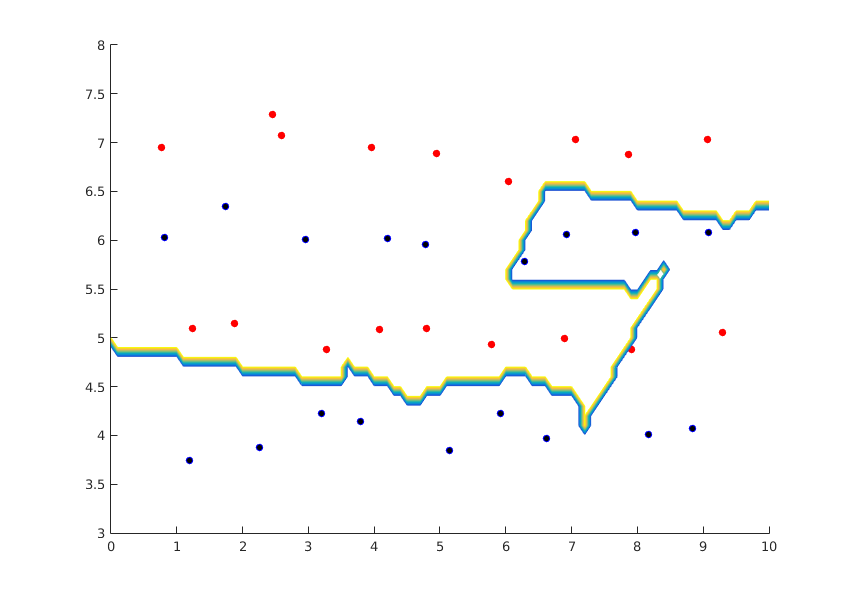
\includegraphics[width=\textwidth]{oldsup}
\caption{Visualização da superfície de separação para o CHIP-CLAS original}
\label{supvelha}
\end{figure}

\begin{figure}[ht]
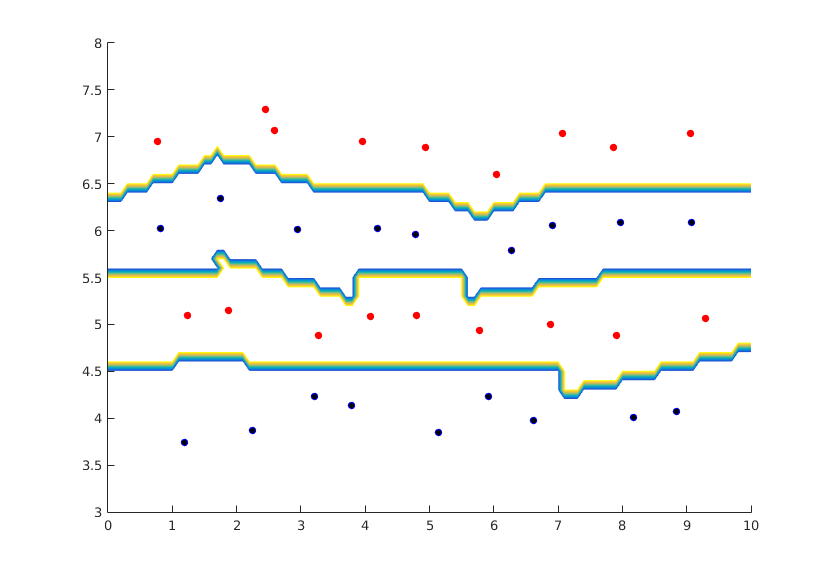
\includegraphics[width=\textwidth]{newsup}
\caption{Visualização da superfície de separação para o AM-CHIP-CLAS}
\label{supnova}
\end{figure}


\subsection{Utilização dos Dados}

A porcentagem dos dados desconsiderados no treinamento para cada execução da validação cruzada foi medida. Calculou-se a razão entre a quantidade de amostras descartadas no processo de filtragem e o total de dados da base, com e sem aprendizado de métrica. Os resultados médios obtidos para as execuções se encontram na Tabela \ref{dltab}.

% latex table generated in R 3.1.3 by xtable 1.8-2 package
% Fri Aug 11 07:56:17 2017
\begin{table}[ht]
\centering
\caption{Porcentagem média desconsiderada dos dados.} 
\label{dltab}
\begin{tabular}{rlrr}
  \hline
 & dataset & CHIP-CLAS & AM-CHIP-CLAS \\ 
  \hline
1 & sonar & 0.00 & 0.00 \\ 
  2 & breastcancer & 15.32 & 10.85 \\ 
  3 & australian & 37.97 & 38.89 \\ 
  4 & diabetes & 44.68 & 44.73 \\ 
  5 & breastHess & 38.94 & 26.16 \\ 
  6 & bupa & 48.28 & 48.76 \\ 
  7 & haberman & 45.97 & 45.24 \\ 
  8 & banknote & 0.00 & 0.00 \\ 
  9 & fertility & 43.11 & 24.78 \\ 
  10 & parkinsons & 10.36 & 3.24 \\ 
  11 & climate & 39.55 & 22.55 \\ 
  12 & ILPD & 47.55 & 47.27 \\ 
  13 & german & 46.86 & 47.30 \\ 
  14 & heart & 43.25 & 43.66 \\ 
  15 & golub & 37.05 & 0.00 \\ 
   \hline
\end{tabular}
\end{table}
\par Para 6 das 15 bases testadas, a porcentagem desconsiderada dos dados diminuiu consideravelmente, sofrendo variação de menos de $1\%$ para cima ou para baixo nas bases restantes. Isto sugere uma maior utilização dos dados para o AM-CHIP-CLAS. A significância estatística desta superioridade pode ser estabelecida através de um teste estatístico de Wilcoxon pareado \cite{Demsar2006}. O teste unilateral foi utilizado, com nível de confiança de $95\%$ ($\alpha = 0.05$). O Valor-p obtido no teste foi $p = 0.040$, de forma que $p < \alpha$, confirmando estatisticamente a maior utilização dos dados para a nova abordagem com $95\%$ de confiança.

\subsection{Desempenho}

A AUC para cada execução da validação cruzada foi medida e foi extraída a média para cada base de dados. Os resultados obtidos se encontram na Tabela \ref{tabauc}, juntamente com a média da posição de cada classificador num \textit{ranking} de desempenho para cada base de dados.

% latex table generated in R 3.1.3 by xtable 1.8-2 package
% Fri Aug 11 07:56:18 2017
\begin{table}[ht]
\centering
\caption{AUC Média das execuções e Rank Médio dos Classificadores.} 
\label{tabauc}
\begin{tabular}{lrrrr}
  \hline
dataset & AM-CHIP-CLAS & CHIP-CLAS & RBF-SVM & Poly-SVM \\ 
  \hline
sonar & 0.84 & 0.88 & 0.84 & 0.87 \\ 
  breastcancer & 0.97 & 0.96 & 0.97 & 0.96 \\ 
  australian & 0.86 & 0.85 & 0.86 & 0.87 \\ 
  diabetes & 0.71 & 0.72 & 0.71 & 0.71 \\ 
  breastHess & 0.83 & 0.81 & 0.76 & 0.77 \\ 
  bupa & 0.58 & 0.61 & 0.67 & 0.72 \\ 
  haberman & 0.54 & 0.56 & 0.52 & 0.50 \\ 
  banknote & 1.00 & 0.99 & 1.00 & 1.00 \\ 
  fertility & 0.50 & 0.59 & 0.50 & 0.50 \\ 
  parkinsons & 0.89 & 0.90 & 0.77 & 0.81 \\ 
  climate & 0.85 & 0.84 & 0.53 & 0.72 \\ 
  ILPD & 0.57 & 0.57 & 0.49 & 0.50 \\ 
  german & 0.70 & 0.67 & 0.66 & 0.68 \\ 
  heart & 0.81 & 0.80 & 0.83 & 0.83 \\ 
  golub & 0.55 & 0.77 & 0.80 & 0.78 \\ 
   \hline
\textbf{Rank Mean} & 2.20 & 2.40 & 2.93 & 2.47 \\ 
   \hline
\end{tabular}
\end{table}
\par Para avaliação estatística dos resultados de múltiplos classificadores, é indicado o teste de Friedman \cite{Demsar2006}. Para um nível de confiança de $95\%$ ($\alpha = 0.05$), foi obtido um Valor-p de $p = 0.445$. O resultado obtido não é suficiente para rejeitar a hipótese nula de que nenhum dos classificadores possui desempenho estatisticamente diferente dos demais. Para melhor visualizar o desempenho dos classificadores, foi feito o teste \textit{post-hoc} de Bonferoni-Dunn \cite{Demsar2006}, obtendo-se o gráfico da Figura~\ref{bonfe}, com o eixo horizontal indicando o \textit{rank} (quanto menor, melhor o desempenho).

\begin{figure}[ht]
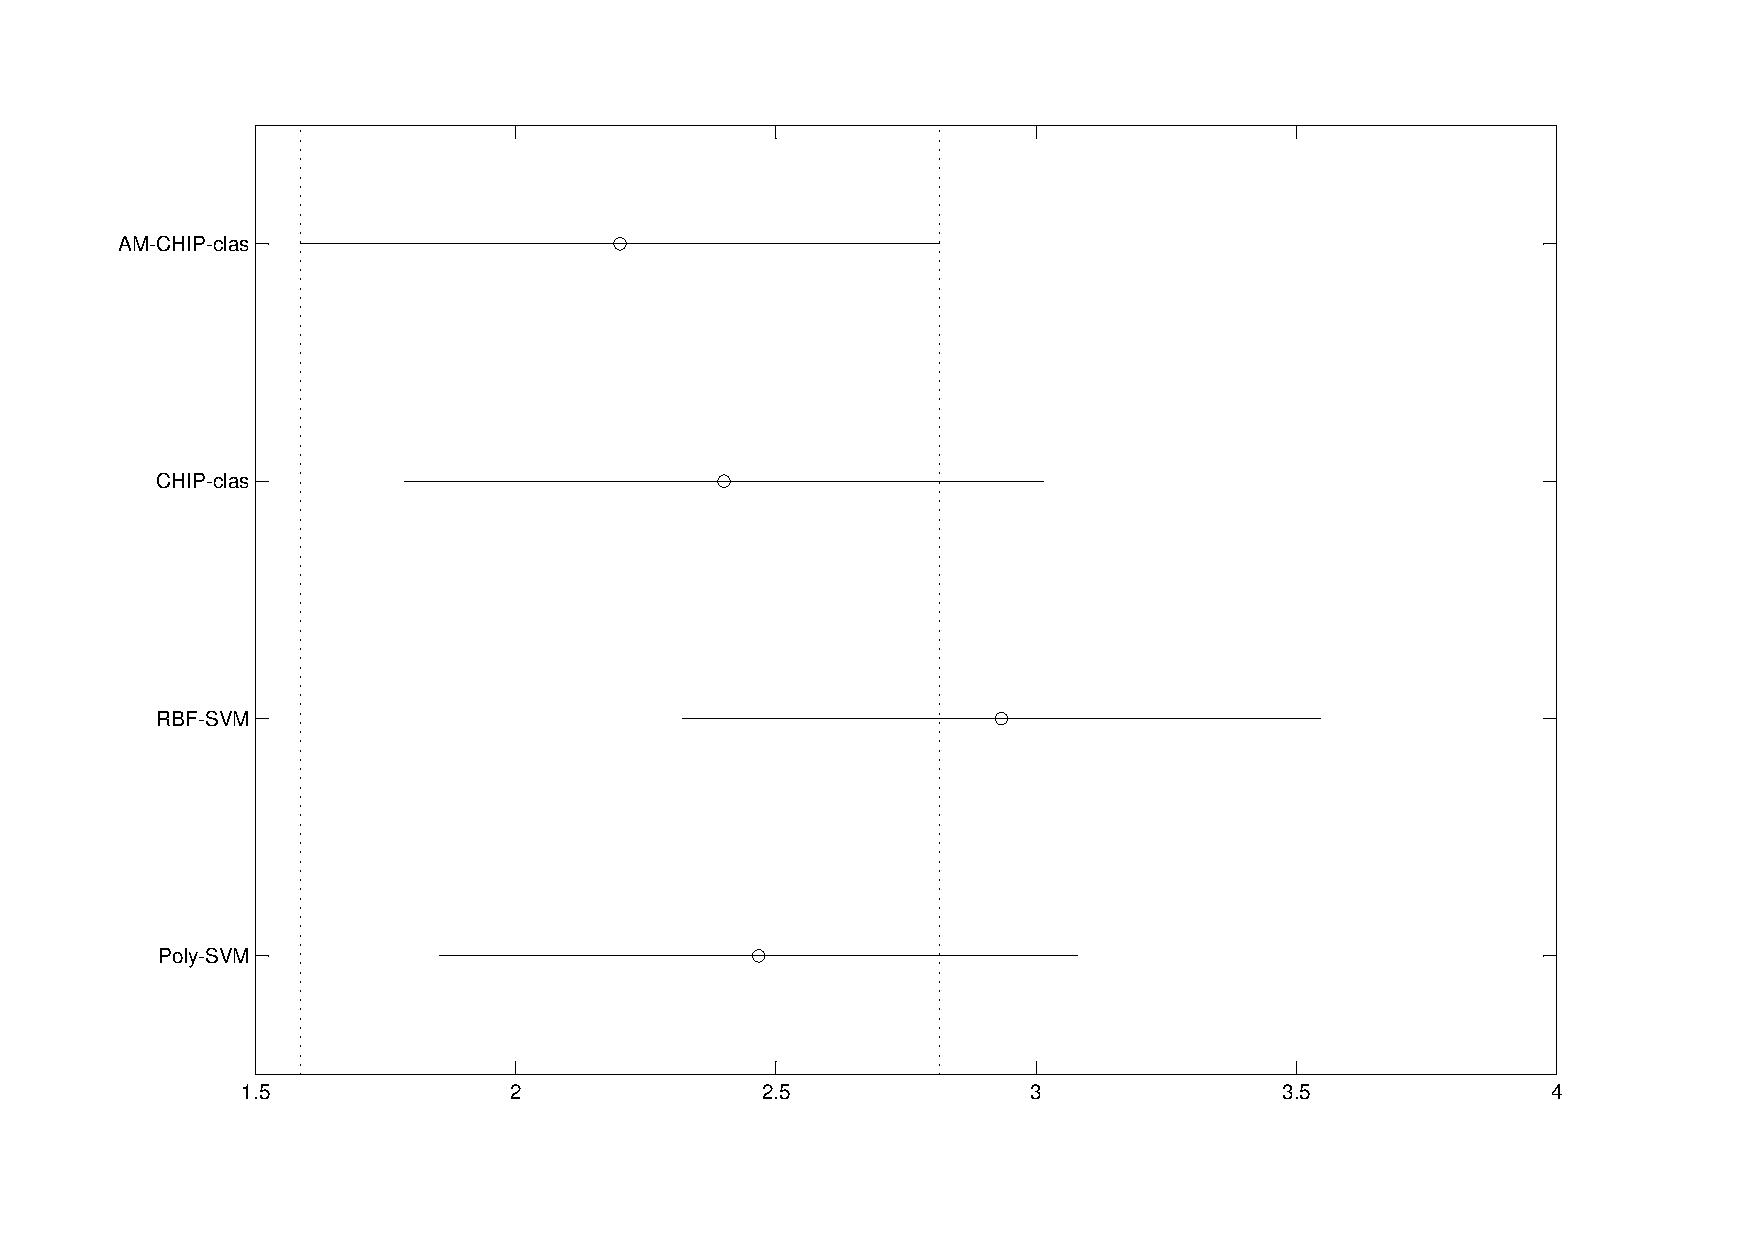
\includegraphics[width=\textwidth]{graf_friedman}
\caption{Visualização para o teste \textit{post-hoc} de Bonferroni-Dunn}
\label{bonfe}
\end{figure}

\par Verifica-se que o desempenho da abordagem AM-CHIP-CLAS não difere significativamente do classificador CHIP-CLAS sem aprendizado de métrica, com \textit{rank} médio pouco superior a este. Ambos CHIP-CLAS e AM-CHIP-CLAS se mostram também superiores no \textit{rank} médio aos classificadores SVM testados, para o \textit{benchmark} utilizado.

% ---
\section{Desempenho}
% ---


% ---
\section{Validação dos Modelos para múltiplos residentes}
% ---

\subsection{Dados para Validação}

Falar sobre o dataset TWOR2010 da WSU.

Para validar o método independentemente da qualidade dos dados coletados, buscou-se na literatura dados oriundos de fontes semelhantes e dispostos em modelo parecido com os dados fornecidos pelo sistema de automaçao residencial da Neocontrol. Foram escolhidos dados divulgados pelo grupo de pesquisa CASAS, da WSU (Washington State University) produzidos ao longo de um ano em uma residência de dois moradores, com anotações do início e do fim de determinadas atividades \cite{Cook2009}. Os dados selecionados provém de um conjunto de 51 sensores de movimento espalhados pela casa e do sensor que detecta abertura da porta principal. Dados presentes na base de dados provenientes de outros sensores foram descartados devido à ausência de correspondência com os dados do sistema da Neocontrol.

\subsection{Resultados}

Mesmo sem o treinamento dos parâmetros, utilizando apenas os valores estimados, o HMM funcionou bem, com suas transicões sendo coerentes com as anotações feitas e com os sensores acionados. Essa coerência foi verificada por inspeção, inspecionando-se 10 sequências de aproximadamente 1000 amostras, 200 antes e 800 depois dos 5 primeiros acionamentos do sensor que detecta abertura da porta principal. Foi verificado visualmente a consistência dos estados com a trajetória plotada na visualização e, no caso de residentes que deixam a casa, as atividades em branco dos sensores. \\
Porém, devido a ausência de um método para identificação dos residentes, resultados improváveis foram observados em momentos onde os mesmos ocupavam o mesmo cômodo. A correção deste problema será objeto de trabalhos futuros.

% ---
\section{Validação da Extração de Características}
% ---

\subsection{Dados para Validação}

Falar sobre o dataset TWOR2010 da WSU.


\subsection{N-Gramas}

O classificador SVM, com características selecionadas através de N-gramas, obteve um resultado, como esperado, pior do que a classificação feita através do algoritmo de Viterbi, alcançando uma precisäo de 80.9\% para um treinamento com 8000 símbolos, porém demorou um tempo consideravelmente menor para obter o resultado, trabalha com um espaço amostral completamente binário e, uma vez treinado, o classificador SVM não precisa dos estados anteriores para realizar as próximas classificações. \\
Nota-se, porém, que a classificação não ultrapassou essa marca, não importa o \textit{gamma} sendo utilizado para o classificador.

\begin{table}[htb]
	\center
	\footnotesize
	\begin{tabular}{llll}
		\textbf{Pred/Obs} & \textbf{0}  & \textbf{1}  & \textbf{2} \\
		\hline
		\textbf{0} & 88\% & 12\% & 0.2\% \\
		\hline
		\textbf{1} & 6\% & 69\% & 25\% \\
		\hline
		\textbf{2} & 2\% & 20\% & 77\% \\
		\hline		
	\end{tabular}
	\caption{Matriz Confusão para resultados obtidos em classificador com \textit{gamma} igual a 0.3}
\end{table}


\subsection{Convolução}


\section{Validação do Algoritmo de Classificação AM-CHIP-CLAS}





\section{Trabalhos Futuros}
% ---

% ----------------------------------------------------------
% Capítulo 5 - Conclusões 1
% ----------------------------------------------------------
\chapter{Conclusão}

Durante o trabalho, foi desenvolvido um meio de se colher dados de utilização de uma casa utilizando tecnologia nacional, em parceria com a indústria. Foram também desenvolvidas formas viáveis de se criar um modelo estatístico HMM destes dados e, a partir deste modelo, a obtenção do estado do modelo para cada observação, eliminando-se a necessidade de anotações para o treinamento supervisionado de algoritmos de classificação sobre o mesmo. Foi também desenvolvido um classificador (N-Gramas+SVM), trabalhando apenas com dados binários no espaço amostral, para classificação destes dados sem necessidade de estados anteriores ou do modelo estatístico após o treinamento. Apesar do desempenho aquém do desejado, a classificação mostrou-se possível.\\
Foi ainda verificada a importância, ao se trabalhar com reconhecimento de padrões, que se utilize ferramentas que levem em conta todas as informaçöes disponíveis sobre os dados. Foi claro durante a execução do projeto a diferença de desempenho dos algoritmos que não faziam assumpção alguma sobre os dados (sem seleção de características) daqueles que levavam em conta o caráter sequencial do mesmo (N-Gramas), e ainda melhor foi o comportamento quando se utilizou um modelo estatístico coerente, criado a partir de informações do sistema monitorado (HMM). \\


% ---
% Finaliza a parte no bookmark do PDF, para que se inicie o bookmark na raiz
% ---
\bookmarksetup{startatroot}% 
% ---

% ----------------------------------------------------------
% ELEMENTOS PÓS-TEXTUAIS
% ----------------------------------------------------------
\postextual

% ----------------------------------------------------------
% Referências bibliográficas
% ----------------------------------------------------------
\bibliography{dissert_ref}

\end{document}
